\section{Problem formulation and system model}
For queue $q$, let $A_q(T)$ be alerts whose ledger-recorded evidence availability minute is at most cutoff $T=100$. Each alert has an identifier, source identifier, observation identifier, event minute, host, account, process context, severity, and asset criticality. A relationship token $r=(a,b)$ is accompanied by claims from process, authentication, and network-flow families. A claim has an observation identifier, upstream-root identifier, optional \texttt{derived\_from} pointer, event-field assertions, and availability minute. Original means the derivation pointer is null; a derived copy remains dependent on its origin.

The algorithm outputs a partition $\mathcal G_q=(G_1,\ldots,G_m)$ of $A_q(T)$, ordered by a deterministic group score. Initial grouping uses source, process-tree, and selected lineage context; the extra verification stage is applied to cross-fragment claim tokens. An edge proposal is evidence for a possible union, whereas a group is a transitive partition component. The simulator's expert priority list and incident assignments are restricted to the evaluator. They are never model-visible fields.

\begin{table}[ht]\centering\footnotesize\caption{Notation used in the method and evaluation.}\label{tab:notation}\begin{tabularx}{\linewidth}{@{}p{22mm}Y@{}}\toprule Symbol & Meaning\\\midrule $q,T$ & Queue and decision cutoff (minute 100 in these experiments)\\ $A_q(T)$ & Eligible alerts whose evidence is available by $T$\\ $r,B_r$ & Relationship token and its visible claim bundle\\ $\rho(c)$ & Upstream origin/root identifier of original claim $c$\\ $\mathcal G_q$ & Ranked partition of eligible alerts\\ $I_q^{20}$ & Twenty expert-priority incidents in queue $q$\\ $Q(i,G)$ & Evaluator qualification of group $G$ for incident $i$\\ $n_i$ & Eligible alert count for incident $i$\\\bottomrule\end{tabularx}\end{table}

Event time represents when the activity occurred; availability time represents when its supporting observation reached the receiver. A claim available at minute 105 is excluded at the minute-100 decision even if its event refers to minute 60.
\begin{figure}[ht]\centering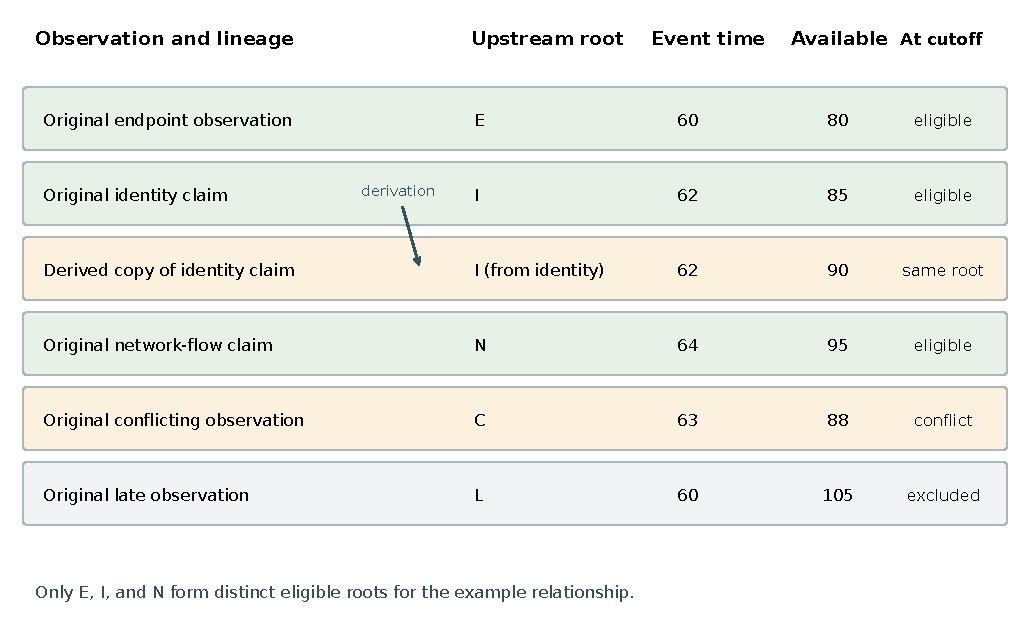
\includegraphics[width=.95\linewidth]{figures/evidence_provenance.pdf}\caption{Schematic point-in-time evidence record with illustrative minute values, not measured holdout observations. The original endpoint, identity, and network observations carry distinct roots E, I, and N. The derived identity copy retains root I, a contradictory observation cannot support the relationship, and an observation made at event minute 60 but available only at minute 105 is invisible at the minute-100 decision. Event time and evidence availability are different fields.}\label{fig:provenance}\end{figure}
